\chapter{Expansión de Friedmann, radiación y materia oscura}

\section{Repaso de la ecuación cosmológica básica}

A escalas mayores que las de los cúmulos de galaxias, se considera que el universo es homogéneo. Elijamos las coordenadas de modo que nosotros estemos en \(x=0\) y situemos una galaxia representativa —o, sencillamente, una partícula imaginaria que se mueve con el flujo de Hubble— en \(x=1\). Por definición, su distancia física respecto de nosotros es entonces el factor de escala \(a(t)\). Un punto en \(x=2\) está a una distancia \(2a(t)\), y así sucesivamente.

\begin{figure}[ht]
\centering
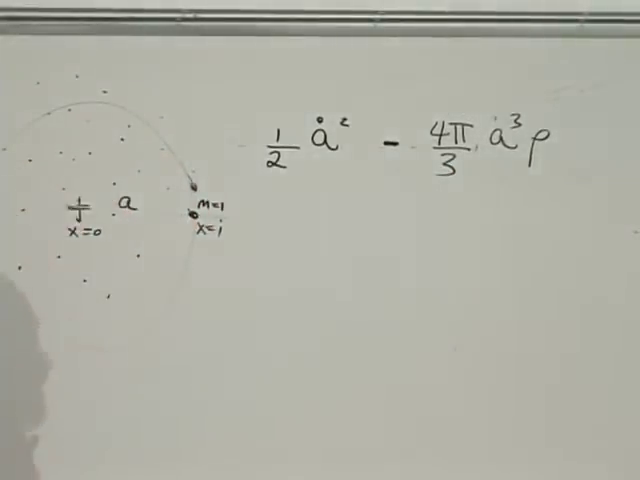
\includegraphics[width=0.78\textwidth]{lecture_03_figure_02.png}
\caption{Esfera homogénea centrada en \(x=0\), una galaxia comóvil en \(x=1\) y el balance de energía newtoniano para \(a(t)\).}
\end{figure}

Solo la materia que está dentro de la esfera de radio \(a(t)\) contribuye a la atracción gravitatoria sobre la partícula en \(x=1\). Asignemos a esa partícula una masa unidad. Su energía cinética es
\begin{equation}
\frac{1}{2}\dot a^2.
\end{equation}
La masa encerrada por la esfera es
\begin{equation}
M_{\mathrm{enc}}=\frac{4\pi}{3}a^3\rho,
\end{equation}
por lo que la energía potencial gravitatoria es
\begin{equation}
-\frac{G M_{\mathrm{enc}}}{a}
=
-\frac{4\pi G}{3}a^2\rho.
\end{equation}
\editorialnote{En la marca de tiempo 00:05:30 de la clase, la pizarra muestra con claridad el término cinético y el término potencial, que depende de la densidad. El coeficiente completo que se escribe aquí se obtiene de la derivación oral.}

La conservación de la energía da
\begin{equation}
\frac{1}{2}\dot a^2-\frac{4\pi G}{3}a^2\rho=\text{const}.
\end{equation}
A continuación, la constante se escribe como \(-k\), con la advertencia habitual de que la normalización estándar solo fija realmente esa notación después de multiplicar la ecuación por \(2\). En la forma estándar,
\begin{equation}
\dot a^2=\frac{8\pi G}{3}a^2\rho-k,
\end{equation}
y al dividir por \(a^2\) se obtiene
\begin{equation}
\left(\frac{\dot a}{a}\right)^2=\frac{8\pi G}{3}\rho-\frac{k}{a^2}.
\end{equation}
Esta es la ecuación de Friedmann en la forma que se utiliza a lo largo de la exposición.

\begin{figure}[ht]
\centering
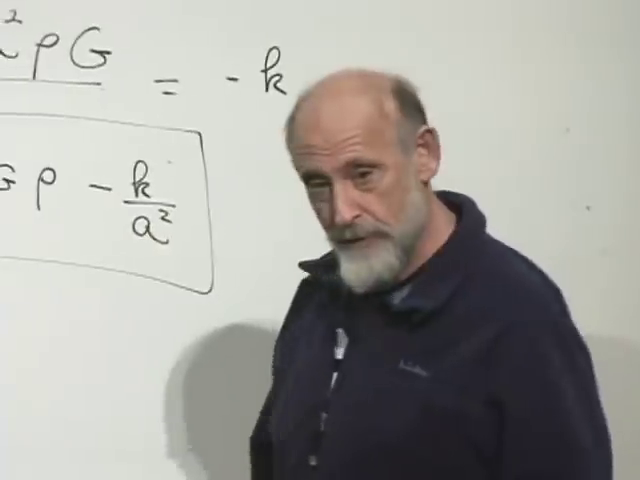
\includegraphics[width=0.56\textwidth]{lecture_03_figure_03.png}
\caption{Contribución de curvatura \(-k/a^2\) aislada en la ecuación de Friedmann.}
\end{figure}

Empíricamente, el término de curvatura es muy próximo a cero; tanto, que a este nivel es muy buena aproximación despreciarlo sin más. Sí corresponde a la curvatura del espacio, pero, desde el punto de vista observacional, aquí es demasiado pequeño incluso para determinar su signo.

La misma ecuación también se obtiene de la relatividad general. Esquemáticamente, la ecuación de Einstein para la componente temporal es
\begin{equation}
R_{00}-\frac{1}{2}g_{00}R \propto T_{00}.
\end{equation}
\editorialnote{Aquí solo se da la estructura tensorial, no el coeficiente numérico global exacto.}
Con una métrica homogénea en expansión, el lado geométrico produce la combinación de \(\dot a/a\) y \(k/a^2\), mientras que el lado de la materia produce la densidad de energía. En esta etapa, el argumento newtoniano y la ecuación de Einstein dicen lo mismo.

Eso también cambia el significado de \(\rho\). De aquí en adelante, es mejor llamar a \(\rho\) la densidad de energía. Para la materia que se mueve lentamente en el sistema comóvil, esta es simplemente la densidad de energía en reposo.

\section{Dominio de la materia}

Supongamos ahora que la densidad de energía se debe a materia en reposo en el sistema comóvil. Consideremos un cubo de una unidad de longitud coordenada por lado. Sus longitudes físicas son \(a(t)\), por lo que su volumen físico es \(a^3(t)\). Si la energía en forma de masa contenida en ese cubo comóvil es \(M\), y la materia se mueve con el flujo en vez de atravesar la frontera, entonces
\begin{equation}
\rho_m=\frac{M}{a^3}.
\end{equation}

Este es el caso dominado por la materia. En esta idealización, las partículas están en reposo dentro de la caja, así que se considera que la temperatura y la presión son cero. Para que haya presión, las partículas tendrían que atravesar la frontera de la caja.

Con \(k\approx 0\), la ecuación queda
\begin{equation}
\left(\frac{\dot a}{a}\right)^2=\frac{8\pi G}{3}\frac{M}{a^3}.
\end{equation}
Probemos una ley potencial,
\begin{equation}
a(t)=Ct^p.
\end{equation}
Entonces
\begin{equation}
\frac{\dot a}{a}=\frac{p}{t},
\end{equation}
De modo que el miembro izquierdo escala como \(t^{-2}\), mientras que el derecho escala como \(t^{-3p}\). Al igualar las potencias se obtiene
\begin{equation}
3p=2,
\qquad
p=\frac{2}{3}.
\end{equation}
Por tanto,
\begin{equation}
a(t)\propto t^{2/3}.
\end{equation}
Al conservar el coeficiente se obtiene
\begin{equation}
C^3=6\pi G M.
\end{equation}

Lo importante de la solución es la ley potencial. Un universo dominado por la materia se expande como la potencia dos tercios del tiempo, no de forma lineal. Esta ley describe una larga etapa intermedia, desde aproximadamente \(10^5\) años después del Big Bang hasta unos pocos miles de millones de años más tarde. El universo actual no está literalmente dominado por la materia, porque ahora domina la energía oscura, pero la materia ordinaria y un largo período de la historia cosmológica se describen de este modo.

\section{Dominio de la radiación}

Antes de esa etapa, la radiación dominaba la densidad de energía. La razón es sencilla. El universo contiene una cantidad enorme de fotones —aproximadamente \(10^9\) por cada protón— y, cuando el universo se comprime, esos fotones adquieren más energía.

Un fotón no tiene masa en reposo, pero sí energía. Su energía es
\begin{equation}
E_\gamma=h\nu=\frac{hc}{\lambda}.
\end{equation}
La hipótesis crucial es que, a medida que el universo se expande, las longitudes de onda de los fotones se estiran con él:
\begin{equation}
\lambda\propto a.
\end{equation}
Una onda dentro de una caja da la imagen adecuada. Si la caja crece, la longitud de onda del modo crece junto con ella. Aquí se aplica la misma idea al universo en expansión.

Como \(\lambda\propto a\), la energía de cada fotón escala como
\begin{equation}
E_\gamma\propto a^{-1}.
\end{equation}
Volvamos a tomar una caja comóvil de una unidad de lado. Los fotones entran y salen, pero, en promedio, el número que hay dentro permanece constante. Así, la energía total de los fotones en la caja también escala como \(a^{-1}\). Al dividirla por el volumen físico \(a^3\), la densidad de energía de la radiación escala como
\begin{equation}
\rho_r\propto a^{-4}.
\end{equation}

Ese factor adicional de \(a^{-1}\) marca toda la diferencia. La materia se diluye porque el universo se expande. La radiación se diluye por esa misma razón y, además, porque cada fotón sufre un corrimiento al rojo.

Por tanto, la ecuación de Friedmann para un universo dominado por la radiación es
\begin{equation}
\left(\frac{\dot a}{a}\right)^2=\frac{8\pi G}{3}\frac{M_r}{a^4}.
\end{equation}
\editorialnote{En la exposición oral se reutiliza el símbolo \(M\) para esta nueva constante. Aquí se añade el subíndice \(r\) solo para evitar confundirla con el caso de la materia.}

Probemos la misma forma \(a(t)=Ct^p\). El miembro izquierdo vuelve a escalar como \(t^{-2}\), mientras que el derecho escala como \(t^{-4p}\). Al igualar las potencias se obtiene
\begin{equation}
4p=2,
\qquad
p=\frac{1}{2}.
\end{equation}
Así que
\begin{equation}
a(t)\propto t^{1/2}.
\end{equation}
Al conservar el coeficiente se obtiene
\begin{equation}
C^4=\frac{32\pi G}{3}M_r.
\end{equation}

\begin{classroomqa}
\lecturetimestamp{00:35:41}
\audiencequestion{¿Por qué aparece un \(G\) ahí?}
\lecturerresponse{Porque lo que gravita es la densidad de energía, no solo la masa en reposo. En el caso de la materia que se mueve lentamente, es fácil pasar por alto la diferencia, pero los fotones nos obligan a tenerla en cuenta: no tienen masa en reposo y, aun así, gravitan.}
\end{classroomqa}

Una caja llena de radiación permite ver la idea con claridad. Empujemos una caja llena de fotones. Cuando la caja acelera, la pared que avanza hacia los fotones recibe impactos más fuertes que la pared que se aleja de ellos, de modo que hay que empujar con más fuerza para vencer la presión de radiación. Por tanto, la caja tiene más inercia y, según el principio de equivalencia, esa inercia adicional también implica más masa gravitatoria. Este es el argumento de la caja de fotones que se emplea aquí para afirmar que la energía gravita.

\begin{classroomqa}
\lecturetimestamp{00:38:11}
\audiencequestion{¿Se puede resolver alguna de estas ecuaciones para un \(a\) que disminuya con el tiempo?}
\lecturerresponse{Sí. Si se reincorpora el término de curvatura \(k/a^2\), hay soluciones en las que el universo se expande y luego se contrae. No parece que eso sea lo que ocurre en nuestro universo, pero la ecuación lo permite.}
\end{classroomqa}

\begin{classroomqa}
\lecturetimestamp{00:38:44}
\audiencequestion{¿Qué pasó con la conservación de la energía?}
\lecturerresponse{Si se reincorpora el término \(k\) y se vuelve a multiplicar la ecuación por \(a^2\), la ecuación cosmológica es precisamente la ley de conservación. La materia o la radiación de un lado son solo una parte del balance. La expansión aporta las partes cinética y gravitatoria, y el balance total se conserva.}
\end{classroomqa}

\section{Materia y radiación juntas}

La cosmología real contiene tanto materia como radiación. Sus densidades escalan de manera distinta:
\begin{equation}
\rho_m\propto a^{-3},
\qquad
\rho_r\propto a^{-4}.
\end{equation}
Así que, para valores pequeños de \(a\), domina la radiación. Para valores grandes de \(a\), domina la materia. Por tanto, al retroceder en el tiempo, se concluye que el universo primitivo estaba dominado por la radiación.

\begin{figure}[ht]
\centering
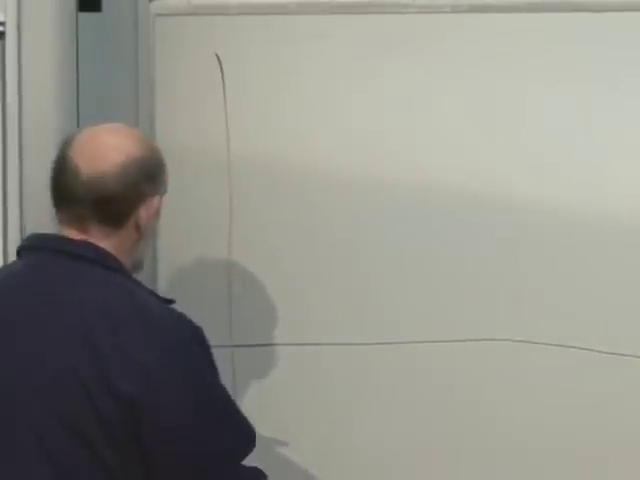
\includegraphics[width=0.68\textwidth]{lecture_03_figure_05.png}
\caption{Ejes para comparar las densidades de energía de la materia y la radiación en función del factor de escala.}
\end{figure}

\editorialnote{En la marca de tiempo 00:44:45 de la clase, la pizarra muestra únicamente los ejes al comienzo de la gráfica comparativa. Las curvas de la materia y la radiación que se analizan inmediatamente después se describen en el texto, pero no se vuelven a dibujar aquí.}

La curva de la materia decrece como \(a^{-3}\). La curva de la radiación decrece como \(a^{-4}\). Ambas divergen cuando \(a\to 0\), pero allí la curva de la radiación crece más deprisa, así que las dos curvas se cruzan en un factor de escala de igualdad. Una estimación aproximada sitúa esta transición después de alrededor de \(10^4\) años, quizá algo más tarde.

La misma idea puede expresarse en la gráfica de \(a(t)\) en función de \(t\). Al principio, la expansión se comporta como \(t^{1/2}\). Más adelante, se comporta como \(t^{2/3}\). El cambio no es un salto, sino una transición continua a lo largo de un intervalo de tiempo relativamente estrecho.

\begin{classroomqa}
\lecturetimestamp{00:44:04}
\audiencequestion{¿La potencia \(p\) pasa de forma continua de \(1/2\) a \(2/3\) a medida que envejece el universo?}
\lecturerresponse{Sí. No hay un salto. El cambio es continuo, aunque ocurre en un intervalo de tiempo bastante estrecho.}
\end{classroomqa}

\section{Temperatura, recombinación y última dispersión}

La siguiente magnitud es la temperatura. Si la energía de un fotón típico escala como \(a^{-1}\), lo mismo ocurre con la temperatura del baño de radiación:
\begin{equation}
T\propto a^{-1}.
\end{equation}
Si \(a\) se duplica, la temperatura se reduce a la mitad.

Tomemos la temperatura actual de los fotones como aproximadamente \(3\,\mathrm K\) y la temperatura de ionización como aproximadamente \(3000\,\mathrm K\), más o menos la temperatura de la superficie del Sol. Entonces
\begin{equation}
\frac{a_{\mathrm{today}}}{a_{\mathrm{ion}}}\sim 10^3.
\end{equation}
Usando la ley de dominio de la materia para tiempos tardíos, \(a\propto t^{2/3}\),
\begin{equation}
\left(\frac{t_{\mathrm{today}}}{t_{\mathrm{ion}}}\right)^{2/3}\sim 10^3,
\end{equation}
por lo que
\begin{equation}
\frac{t_{\mathrm{today}}}{t_{\mathrm{ion}}}\sim 1000^{3/2}\sim 3\times 10^4.
\end{equation}
Si para esta estimación tomamos que la edad del universo es \(10^{10}\) años, obtenemos
\begin{equation}
t_{\mathrm{ion}}\sim 3\times 10^5\ \mathrm{years}.
\end{equation}

Esta es la época en que el hidrógeno y el helio dejan de estar completamente ionizados. Antes de entonces, el universo es un plasma caliente. ¿Por qué es opaco un plasma? Porque las cargas libres responden con fuerza a las ondas electromagnéticas. El campo eléctrico hace oscilar las cargas, el medio se comporta como un conductor y los conductores son opacos. Esa es la analogía pertinente con la superficie del Sol.

Cuando el universo se enfría lo suficiente para que los electrones se recombinen con los núcleos, se forman átomos neutros ordinarios y el universo se vuelve mucho más transparente. La transición no es infinitamente abrupta. Ocurre en una región o un intervalo de tiempo difusos, pero es lo bastante definida para la cosmología como para llamarla superficie de última dispersión.

Mirar hacia el exterior significa mirar hacia atrás en el tiempo. Las galaxias cercanas muestran el pasado reciente. Las galaxias más lejanas muestran épocas anteriores. A suficiente distancia, todas las líneas de visión llegan a la época en que el universo aún estaba ionizado y era opaco. La radiación electromagnética no puede mostrarnos nada anterior a esa época.

En principio, otros mensajeros podrían permitir explorar épocas anteriores. Los neutrinos son eléctricamente neutros y se desacoplarían antes. Los gravitones, si algún día se pudieran observar, procederían de épocas aún más tempranas. Pero la misma debilidad de la interacción que les permitiría atravesar el plasma primitivo también los hace extremadamente difíciles de detectar.

Si en algún momento el universo estuvo tan caliente como la superficie del Sol en todas direcciones, ¿por qué el cielo no brilla con una intensidad cegadora? Porque la superficie de última dispersión se aleja, y los fotones que nos llegan desde ella han sufrido un corrimiento al rojo por un factor aproximadamente igual a \(10^3\), que es la razón entre \(3000\,\mathrm K\) y \(3\,\mathrm K\). Lo que nos llega es radiación de microondas, no luz solar visible.

\begin{classroomqa}
\lecturetimestamp{01:03:51}
\audiencequestion{¿Entonces nuestros telescopios no pueden observar épocas anteriores a unos \(300{,}000\) años?}
\lecturerresponse{Los telescopios electromagnéticos no pueden. Antes de esa época, el universo estaba ionizado y era opaco. En principio, otros mensajeros podrían permitir explorar épocas anteriores.}
\end{classroomqa}

\begin{classroomqa}
\lecturetimestamp{01:08:43}
\audiencequestion{Cuando hablas de la temperatura de un fotón, te refieres a la temperatura de un cuerpo negro cuya radiación tiene ese pico. Pero no depende linealmente de la longitud de onda, ¿verdad?}
\lecturerresponse{Exacto. La temperatura corresponde, en esencia, a la energía de un fotón típico, de modo que, para un fotón, es inversamente proporcional a la longitud de onda. La ley \(T^4\) se refiere a la densidad de energía, no a la energía de un solo fotón. Combina la energía por fotón con el número de fotones por unidad de volumen, y la densidad numérica escala como \(T^3\).}
\end{classroomqa}

Por tanto,
\begin{equation}
n_\gamma\propto T^3,
\qquad
\rho_\gamma\propto T^4.
\end{equation}

\section{Materia oscura a partir de las curvas de rotación}

La materia oscura aparece al estudiar las curvas de rotación galácticas. No se infirió a partir de la ecuación de Friedmann a gran escala, sino de observaciones astronómicas a escala galáctica.

Empecemos con el problema newtoniano más sencillo: un cuerpo ligero de masa \(m\) que orbita una masa central \(M\) a un radio \(r\). La fuerza gravitatoria es
\begin{equation}
\frac{GMm}{r^2},
\end{equation}
y la aceleración centrípeta es \(v^2/r\). La ley de Newton da
\begin{equation}
m\frac{v^2}{r}=\frac{GMm}{r^2}.
\end{equation}
Se simplifica \(m\), se multiplica por \(r\) y se obtiene
\begin{equation}
v(r)=\sqrt{\frac{GM}{r}}.
\end{equation}
Así que, si la masa gravitatoria está concentrada cerca del centro, la velocidad orbital decrece como \(r^{-1/2}\).

Eso es lo que cabría esperar si la masa siguiera la luz. La mayor parte de la materia visible de una galaxia se encuentra cerca del núcleo, así que, en ese caso, las estrellas exteriores se comportarían de forma muy parecida a los planetas de las regiones externas del sistema solar. Los astrónomos infieren las velocidades orbitales midiendo las diferencias de corrimiento Doppler a través de una galaxia cercana: comparan el lado que se mueve hacia nosotros con el que se aleja, una vez descontado el movimiento recesivo global de la galaxia. Las velocidades orbitales medidas se mantienen aproximadamente constantes hasta radios grandes.

Así que sustituyamos la masa central \(M\) por la masa encerrada \(M(r)\):
\begin{equation}
\frac{v^2}{r}=\frac{G M(r)}{r^2}.
\end{equation}
Si \(v(r)\) es aproximadamente constante, entonces
\begin{equation}
M(r)\propto r.
\end{equation}
En otras palabras, la masa gravitatoria sigue aumentando con el radio incluso en regiones donde la luz visible no lo hace.

Supongamos ahora, como se hace por simplicidad en la exposición, que la distribución de masa es aproximadamente esférica. Entonces
\begin{equation}
M(R)=\int_0^R 4\pi r^2\rho(r)\,dr.
\end{equation}
Si \(M(R)\propto R\), al derivar con respecto a \(R\) se obtiene
\begin{equation}
4\pi R^2\rho(R)\propto 1,
\end{equation}
y, por tanto,
\begin{equation}
\rho(r)\propto \frac{1}{r^2}.
\end{equation}

\begin{classroomqa}
\lecturetimestamp{01:28:18}
\audiencequestion{Parece que la densidad debería variar como \(1/r^2\). ¿Hay alguna razón para ello?}
\lecturerresponse{A partir de la curva de rotación plana observada se infiere \(M(R)\propto R\), y al derivar se obtiene \(\rho(r)\propto 1/r^2\). Más allá de eso, aquí no se propone ninguna explicación sencilla basada en primeros principios; las simulaciones detalladas hacen gran parte del trabajo.}
\end{classroomqa}

La conclusión firme es que una galaxia contiene mucha más masa gravitatoria de la que sugeriría la materia luminosa por sí sola: varias veces más y, según la estimación utilizada aquí, aproximadamente un orden de magnitud más. La galaxia visible está dentro de un halo oscuro mucho mayor.

¿Qué impide que el gas ordinario permanezca en un estado tan difuso? La disipación. Una nube de gas se contrae porque las colisiones, los procesos similares a la fricción y la radiación le permiten perder energía. Al parecer, la materia oscura no emite una cantidad apreciable de radiación y es casi no colisional. La gravedad puede atraerla hacia dentro y convertir energía potencial en energía cinética, pero, sin una disipación eficiente, no colapsa para formar las estructuras luminosas compactas que forma la materia ordinaria. Lo que mantiene extendido el halo es la energía cinética.

A continuación se analizan con cautela varias alternativas. Se dice que los neutrinos son demasiado rápidos para comportarse así a escala galáctica. Un halo compuesto de hidrógeno ordinario alteraría gravemente la nucleosíntesis del universo primitivo. También se menciona que los agujeros negros formados por materia ordinaria plantean problemas, porque implicarían demasiada materia ordinaria en el universo primitivo y suscitarían problemas de lente gravitatoria; la exposición no afirma nada más en ese momento.

El halo no se describe como una cáscara delgada ni como un toro. Es una distribución aproximadamente esférica y no uniforme, más densa hacia el centro y cada vez menos densa hacia el exterior.

\begin{classroomqa}
\lecturetimestamp{01:53:12}
\audiencequestion{¿Te refieres al Cúmulo Bala?}
\lecturerresponse{Sí. El gas de rayos X muestra la materia ordinaria, mientras que las lentes gravitatorias muestran la masa gravitatoria total. En la colisión, esas dos distribuciones se separan. Es una prueba sólida de que la materia oscura es real, y no una mera modificación de la gravedad vinculada exclusivamente a la materia visible.}
\end{classroomqa}

Ese es el último punto observacional. Se sabe muy poco en detalle sobre qué es la materia oscura, pero nada de lo expuesto requiere un principio radicalmente nuevo. La posibilidad más conservadora es, sencillamente, que la naturaleza contenga partículas adicionales que interactúan débilmente y que aún no se han identificado.
